\qns{A slalom problem}

A skier must slide from left to right by going through $n$ parallel gates of known position $(x_i,y_i)$ and width $c_i$, $i=1,\dots,n$. The initial position $(x_0,y_0)$ is given, as well as the final one, $(x_{n+1},y_{n+1})$.
% Here, the $x$-axis represents the direction down the hill, from left to right; and 
Before reaching the final position, the skier must go through gate $i$ by passing between the points $(x_i, y_i - c_i/2)$ and $(x_i, y_i + c_i/2)$ for each $i \in \{1, \dots, n\}$. See Figure~\ref{fig:slalom_pic.pdf}. 


\begin{figure}[h]
\begin{center}
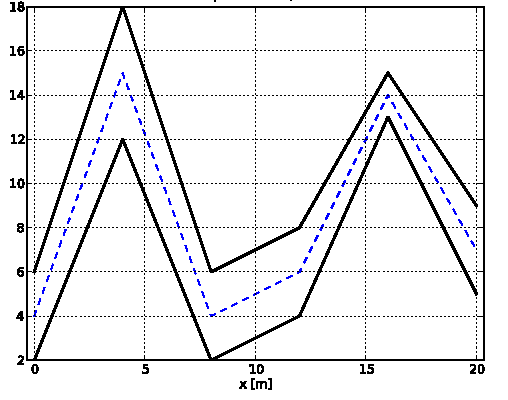
\includegraphics{figures/slalom_pic.pdf} 
%[width=.45\textwidth,height=.25\textheight,angle=0]
\end{center}
\caption{\label{fig:slalom_pic.pdf}  Slalom problem with $n=6$ gates. The initial and final positions are fixed and not included in the figure. The skier slides from left to right. The middle path is dashed and connects the center points of gates.}
\end{figure}

\begin{table}[h]
\caption{Problem data for Problem 2.}
\begin{center}
\[
\begin{array}{c|ccc}
i & x_i & y_i & c_i \\\hline
0 & 0 & 4 & N/A \\
1 & 4 & 5 & 3 \\
2 & 8 & 4 & 2 \\
3 & 12 & 6 & 2 \\
4 & 16 & 5 & 1 \\
5 & 20 & 7 & 2 \\
6 & 24 & 4 & N/A
\end{array}
\]
\end{center}
\label{tab:qplp-data-slalom}
\end{table}
\begin{enumerate}
\item {[Optimization Problem Expression]} Given the data $\{(x_i, y_i, c_i)\}_{i=0}^{n+1}$, write an optimization problem that minimizes the total length of the path. Your answer should come in the form of an SOCP. 
\newline
\newline
\newline
\newline
\sol{\item $g(x_1,x_2) = \dfrac{x_1^2}{4} + \dfrac{x_2^2}{9}$


}
\newline
\item Solve the problem numerically with the data given in Table~\ref{tab:qplp-data-slalom}.
\newline
\sol{\item Show that the following inequalities hold for any vector $x \in \Real{n}$:
\[
% \|x\|_\infty \le \|x\|_1 \le n \|x\|_\infty \\
% \|x\|_2 \le \|x\|_1 \le \sqrt{n} \|x\|_2 \\
% \|x\|_\infty \le \|x\|_2 \le\sqrt{n}\|x\|_\infty \\
\frac{1}{\sqrt{n}}\|x\|_2 \leq \|x\|_\infty \leq  \|x\|_2 \leq \|x\|_1 \leq \sqrt{n} \|x\|_2 \le n\|x\|_\infty.
\]

\textit{Hint:} For $\|x\|_1\leq \sqrt{n}\|x\|_2$, how might you express $\|x\|_1$ as the dot product of two vectors? Can you then use the Cauchy-Schwarz inequality to bound this dot product?}
\newline
\end{enumerate}